\documentclass[usepdftitle=false]{beamer}
\hypersetup{pdftitle=Internationalized Domain Name Homograph Attacks}
\usepackage{graphicx}

\mode<presentation>
{
  \usetheme{default}
  \usecolortheme{default}
  \usefonttheme{default}
  \setbeamertemplate{navigation symbols}{}
  \setbeamertemplate{caption}[numbered]
}
\usepackage[english]{babel}
\usepackage[utf8x]{inputenc}

\title{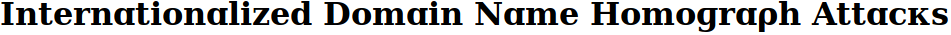
\includegraphics[width=0.8\linewidth]{title}}
\author{Chen Lai, Zhongrong Jian, J. Sidrach}
\institute{University of California San Diego}
\date{CSE 227: Computer Security - Spring 2017}

\begin{document}

\begin{frame}
  \titlepage
\end{frame}

% Uncomment these lines for an automatically generated outline.
%\begin{frame}{Outline}
%  \tableofcontents
%\end{frame}

\begin{frame}{Internationalized Domain Name Homograph Attacks}
\begin{itemize}
  \item Domains registered with Punycode (xn-- prefix)
  \item Displayed in Unicode in browsers' navigation bar
  \item What could go wrong?
  \item \textit{Some} of the Unicode homoglyphs of a, b, c:

  \centering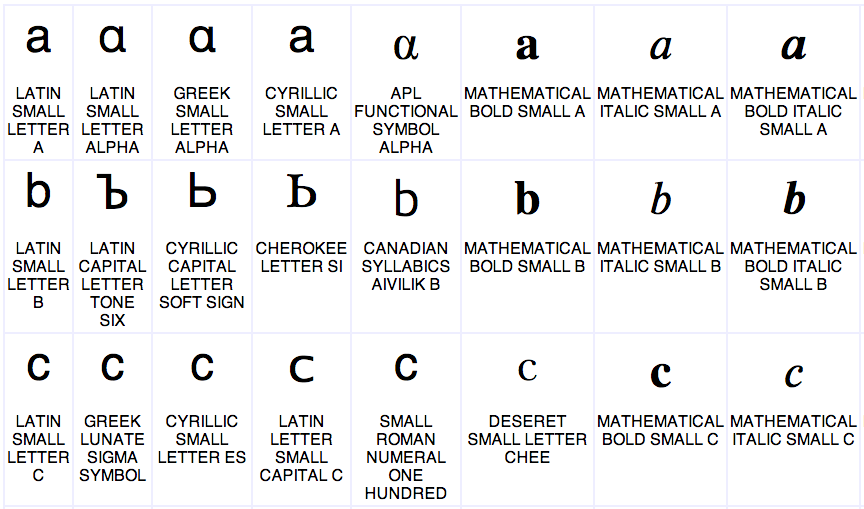
\includegraphics[width=0.8\linewidth]{images/homoglyphs}

  \small{(Image provided by Google)}
\end{itemize}

\end{frame}

\begin{frame}{Defense Mechanisms - Browsers}
\begin{itemize}
\item URLs displayed in Punycode if certain checks fail
\item No common policy across major browsers
\item Successful attack

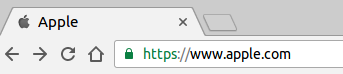
\includegraphics[width=0.4\linewidth]{images/apple}
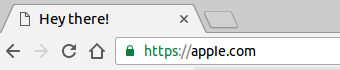
\includegraphics[width=0.4\linewidth]{images/fakeapple-punycode}

\item Unsuccessful attack

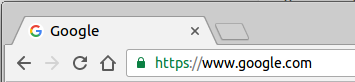
\includegraphics[width=0.4\linewidth]{images/google}
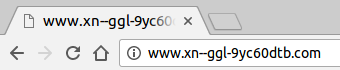
\includegraphics[width=0.4\linewidth]{images/fakegoogle-punycode}
\end{itemize}

\end{frame}

\begin{frame}{Defense Mechanisms - ICANN and TLD Registrars}
ICANN
\begin{itemize}
  \item Rejects ccTLD applications that look similar to existing ones
  \item Does not enforce restrictions to second-level domains
\end{itemize}
TLD Registrars
\begin{itemize}
  \item No common public policy to deal with homograph domains
  \item Notable exception: Chinese TLDs (simplified/traditional)
\end{itemize}
\end{frame}

\begin{frame}{Methodology - Clustering}
Data sources
\begin{itemize}
  \item \textit{.com} zone snapshot
  \item Alexa Top 1 million web sites ranking
\end{itemize}
Clustering Process
\begin{itemize}
  \item Filter IDNs from snapshot
  \item Filter non-IDNs from Alexa ranking
  \item Cluster all homograph IDNs, using a non-IDN homograph domain from the Alexa ranking as the representative
\end{itemize}
\end{frame}

\begin{frame}{Methodology - Classification}
Manual classification using
\begin{itemize}
  \item WHOIS records
  \item HTTP/HTML responses
\end{itemize}
Categories
\begin{itemize}
  \item Canonical - Parking
  \item Canonical - Redirect
  \item Third Party - Redirect to Canonical
  \item Third Party - Unrelated
  \item Third Party - Parking
  \item Third Party - Scam
\end{itemize}
\end{frame}

\begin{frame}{Results (1)}
\begin{table}
\centering
\begin{tabular}{lrr}
\hline
Domains                                           & \#                         & \%                         \\ \hline
\itshape\sffamily{Canonical domain names}         & \itshape\sffamily{458731}  & \itshape\sffamily{8.31\%}  \\
\hspace{0.5cm} With IDN homographs                & 825                        & 6.04\%                     \\
\hspace{0.5cm} Without IDN homographs             & 457906                     & 2.27\%                     \\
\itshape\sffamily{Internationalized Domain Names} & \itshape\sffamily{1045400} & \itshape\sffamily{91.69\%} \\
\hspace{0.5cm} With canonical homograph           & 1099                       & 3.68\%                     \\
\hspace{0.5cm} Without canonical homograph        & 1044301                    & 2.74\%                     \\ \hline
\end{tabular}
\caption{Overview of the clustering results.}
\end{table}
\end{frame}

\begin{frame}{Results (2)}
\begin{table}
\centering
\begin{tabular}{lr}
\hline
Domain       & \# of IDN homographs \\ \hline
google.com   & 24                   \\
youtube.com  & 3                    \\
facebook.com & 9                    \\
baidu.com    & 3                    \\
yahoo.com    & 4                    \\
reddit.com   & 1                    \\
qq.com       & 2                    \\
taobao.com   & 1                    \\
live.com     & 1                    \\
vk.com       & 6                    \\ \hline
\end{tabular}
\caption{Top ten .com domains in the Alexa ranking with IDN homographs.}
\end{table}
\end{frame}

\begin{frame}{Results (3)}
\begin{table}
\centering
\begin{tabular}{lrr}
\hline
Status                               & \#                     & \%                         \\ \hline
\itshape\sffamily{Canonical}         & \itshape\sffamily{88}  & \itshape\sffamily{8.31\%}  \\
\hspace{0.5cm} Parking               & 64                     & 6.04\%                     \\
\hspace{0.5cm} Redirect              & 24                     & 2.27\%                     \\
\itshape\sffamily{Third Party}       & \itshape\sffamily{971} & \itshape\sffamily{91.69\%} \\
\hspace{0.5cm} Redirect to Canonical & 39                     & 3.68\%                     \\
\hspace{0.5cm} Unrelated             & 29                     & 2.74\%                     \\
\hspace{0.5cm} Parking               & 872                    & 82.34\%                    \\
\hspace{0.5cm} Scam                  & 31                     & 2.93\%                     \\ \hline
\end{tabular}
\caption{Breakdown of the manually classified homograph IDNs.}
\end{table}
\end{frame}

\begin{frame}{Results (4)}
\begin{table}
\tiny
\centering
\begin{tabular}{llr}
\hline
Registrant organization              & Registrant email           & \# of Homograph IDNs \\ \hline
Domains By Proxy, LLC                & --                         & 89                   \\
Super Privacy Service c/o Dynadot    & privacy@dynadot.com        & 23                   \\
Domain Registries Foundation         & --                         & 22                   \\
Duong Thien                          & thiendv@outlook.com        & 18                   \\
Syngenuity Limited                   & manager@syngenuity.com     & 12                   \\
Helpnet: Brand Development \& Sales  & help@strongestbrands.com   & 12                   \\
ONUNO L.L.C.                         & corucas@gmail.com          & 11                   \\
Privacy Protection Service INC d/b/a & contact@privacyprotect.org & 10                   \\
Hubertus Henz                        & hu\_h5@yahoo.de            & 9                    \\
wuyu                                 & wy65535@126.com            & 7                    \\ \hline
\end{tabular}
\caption{Top ten registrants with the most homograph IDNs.}
\end{table}
\end{frame}

\begin{frame}{Conclusions}
Current state
\begin{itemize}
  \item No common TLD policies in place
  \item 1000+ homograph IDNs detected
  \item Most domains inactives (parking)
  \item No guarantees they will stay parked in the future
\end{itemize}
Future work
\begin{itemize}
  \item Analyze other TLDs
  \item Improve homograph matching algorithm (OCR?)
  \item Automatic classification of homograph IDNs
\end{itemize}
\end{frame}

\begin{frame}
\centering Q \& A
\end{frame}

\end{document}
